\documentclass[tikz]{standalone}
\usepackage{tikz,amsmath}
\usetikzlibrary{calc}
\begin{document}
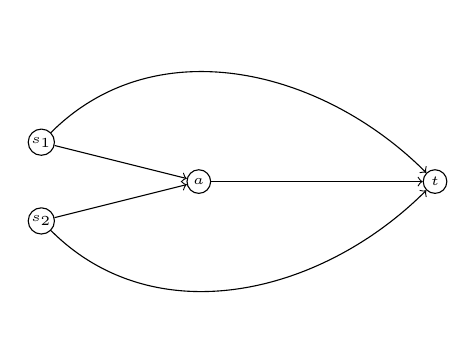
\begin{tikzpicture}[every node/.style={draw,shape=circle, inner sep=.5pt, minimum size=.3cm}]
    \draw (0,0) node (s2) {\tiny{$s_2$}};
    \draw (0,1) node (s1) {\tiny{$s_1$}};
    \draw (2,.5) node (m1) {\tiny{$a$}};
    \draw (5,.5) node (t) {\tiny{$t$}};
    \draw [->] (s1) -- (m1);
    \draw [->] (s2) -- (m1);
    \draw [->] (m1) -- (t);
    \draw (s2) edge[out=-45,in=-135,->]  (t);
    \draw (s1) edge[out=45,in=135,->]  (t);
\end{tikzpicture}
\end{document}
